\documentclass{article}

%--------------------------------------------------------------
% Document & Font Setup
%--------------------------------------------------------------
\usepackage[a4paper, margin=1in]{geometry}
\usepackage{setspace}
\usepackage{parskip}
%--------------------------------------------------------------
% Common Packages
%--------------------------------------------------------------
\usepackage{graphicx}
\usepackage{subcaption}
\usepackage{caption}
% Subfigure captions
\DeclareCaptionLabelFormat{custom}{\figurename~\thefigure~(#2)}
\captionsetup[subfigure]{labelformat=custom}

\usepackage{enumitem}
\usepackage{float}
\usepackage{placeins}
\usepackage[dvipsnames,x11names,svgnames]{xcolor}
\usepackage{url}

%--------------------------------------------------------------
% Math & Science Packages
%--------------------------------------------------------------
\usepackage{amsmath,amssymb,amsfonts,amsthm}
\usepackage{mathtools}
\usepackage{bbm}
\usepackage{siunitx}
\DeclareSIUnit{\rpm}{RPM}
\DeclareSIUnit{\au}{AU}

%--------------------------------------------------------------
% Hyperlinks
%--------------------------------------------------------------
\usepackage{hyperref}
\hypersetup{
    hidelinks,
    colorlinks=true,
    linkcolor=blue,
    urlcolor=red
}

%--------------------------------------------------------------
% Headers & Footers
%--------------------------------------------------------------
\usepackage{fancyhdr, lastpage}

\fancypagestyle{mainmatter}{
    \fancyhf{}
    \lhead{2025}
    \rhead{EPSRC}
    \cfoot{Page \thepage\ of \pageref{LastPage}}
    \renewcommand{\headrulewidth}{0.4pt}
    \renewcommand{\footrulewidth}{0.4pt}
}

%--------------------------------------------------------------
% Todo
%--------------------------------------------------------------
\usepackage{todonotes}

%--------------------------------------------------------------
% Plots & Graphics
%--------------------------------------------------------------
\usepackage{pgfplots}
\pgfplotsset{compat=1.18}
\usepackage{tikz}

% TikZ
\usetikzlibrary{
    shapes.geometric,
    shapes.misc,
    arrows.meta,
    positioning,
    matrix,
    calc,
    fit,
    fadings,
    patterns,
    plotmarks,
    decorations.pathmorphing
}
\tikzset{font={\fontsize{10pt}{12}\selectfont}}
\tikzset{
    startstop/.style = {rectangle, rounded corners, ...},
    IO/.style        = {ellipse, ...},
    arrow/.style     = {thick,->,>={Stealth}},
    block/.style     = {rectangle, draw, ...},
    sum/.style       = {draw, circle, ...},
    bag/.style       = {align=left}
}

% Custom colors
\definecolor{sandybrown}{rgb}{0.96, 0.64, 0.38}

%--------------------------------------------------------------
% Custom Commands, Environments, & Numbering
%--------------------------------------------------------------
\numberwithin{equation}{section}
\numberwithin{figure}{section}
\numberwithin{table}{section}
\numberwithin{algorithm}{section}

\newtheorem{property}{Property}[section]
\newtheorem{theorem}{Theorem}[section]
\newtheorem{corollary}{Corollary}[section]
\newtheorem{definition}{Definition}[section]
\newtheorem{assumption}{Assumption}[section]

\DeclareMathOperator*{\argmax}{arg\,max}
\DeclareMathOperator*{\argmin}{arg\,min}
\newcommand{\defeq}{\vcentcolon=}
\newcommand{\traj}{\{x(k)\}_{k=0,\dots,T}}
\newcommand{\dgap}{d}
\newcommand\given[1][]{\:#1\vert\:}

\let\oldemptyset\emptyset
\let\emptyset\varnothing

\newcommand\blfootnote[1]{%
  \begingroup
  \renewcommand\thefootnote{}\footnote{#1}%
  \addtocounter{footnote}{-1}%
  \endgroup
}
\usepackage[backend=bibtex, sorting=none]{biblatex}
\addbibresource{bibliography.bib}


\title{Project 1: Empirical Observation of the Starlink-3988 Satellite}
\author{Claudio Vestini}


\begin{document}

\maketitle

\section{Introduction \& Satellite Selection}

Since the first successful deployment of a human-made object into Earth's orbit with \textit{Sputnik 1} in 1957, over 15,000 satellites have been placed in orbit around our planet~\cite{lookup-lepoint2025}. Of these, more than 13,000 remain operational today, and this unprecedented active percentage is continuously growing. The vast majority are of American origin (roughly \SI{74}{\percent}), and most belong to SpaceX's Starlink constellation, which alone accounts for approximately \SI{86}{\percent} of all U.S. satellites and \SI{64}{\percent} of the world's total active population. Engineered to provide high-speed, low-latency internet connectivity to underserved rural areas of the world for a moderate service price, Starlink has been rapidly expanding its constellation, with thousands of new satellites being launched every year through proprietary SpaceX vehicles.

\begin{figure}[h!]
    \centering
    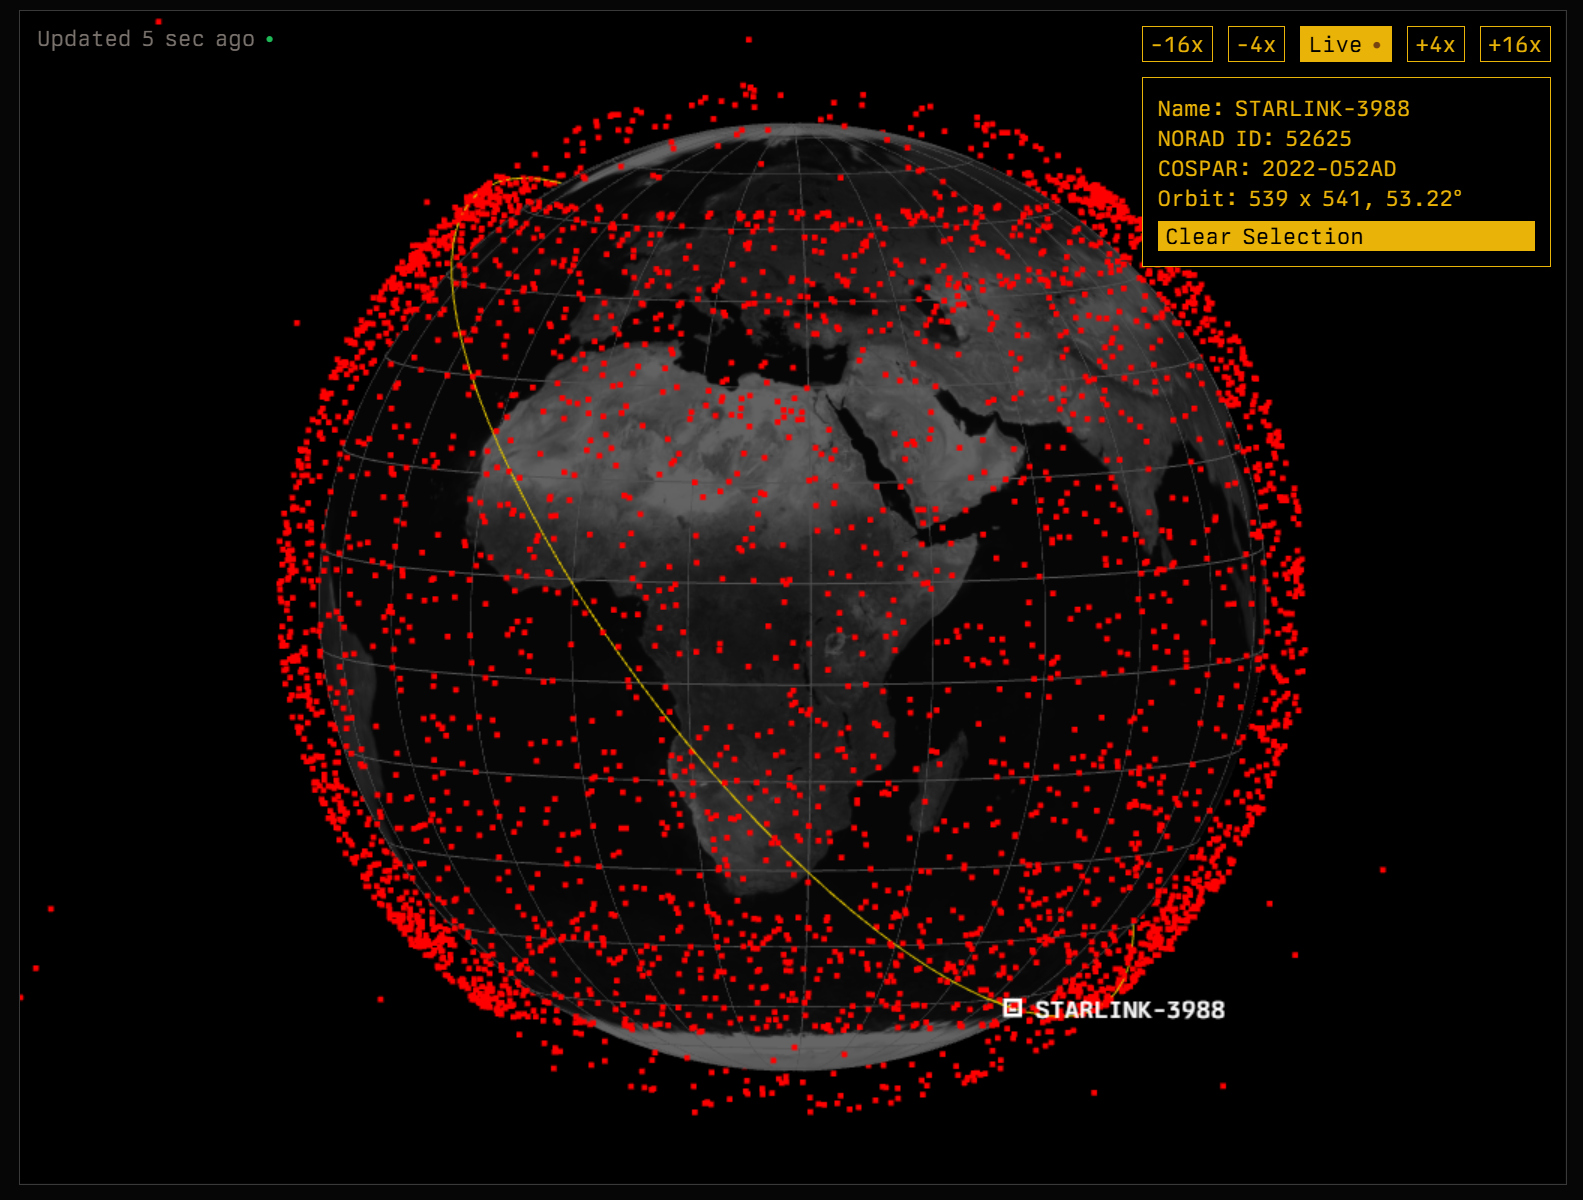
\includegraphics[width=\textwidth]{LaTeX/Figures/Starlink Constellation.png}
    \caption{Starlink constellation as of October 19th 2025, 16:59:33. Each red square represents an active satellite. Highlighted in yellow is the orbital track of selected satellite \textit{Starlink-3988}, with relevant orbital information displayed. The image is a screenshot from the Starlink Map website~\cite{starlinkmap.org}.}
    \label{fig:constellation}
\end{figure}

These satellites have already been used for several key applications, including enabling WiFi connectivity in commercial airlines and cruises, providing life-critical broadband in hurricane-ravaged coastal towns and earthquake-shaken regions, and facilitating allied command and control operations in the Russo-Ukrainian War. The constellation includes nearly 9,700 satellites (as of the writing of this report), and is visualised in Figure~\ref{fig:constellation}. Each unit is equipped with four beamforming, phased array antennas, each of which electronically steers the \SI{11.7}{\giga\hertz} collimated downlink signals in real time to a \SI{24}{\kilo\metre}-diameter ground coverage cell that can serve up to 8,000 simultaneous customers. Furthermore, the satellites communicate with one another via five on-board optical lasers at vacuum light-speed, enabling lower effective latencies between far-away cities compared to underwater cables. This is particularly relevant for applications in stock market trading, where saving a few milliseconds in latency can have a huge impact on the decision-making reactions to market fluctuations. To add to the list of groundbreaking engineering innovations that SpaceX developed for Starlink satellites, the orbital insertion procedure is entirely novel: the satellites are deployed in clusters of up to 23 units\footnote{For the larger v2 model, down from up to 60 units of the smaller v1/v1.5 model} at an altitude of roughly \SI{280}{\kilo\metre}, as shown in Figure~\ref{fig:starlink_cluster}; their orbits are then slowly raised to around \SI{550}{\kilo\metre} in two stages using Kripton gas ion thrusters\footnote{This is a more cost-efficient alternative to the customary option, Xenon gas}. This unusual manoeuvre leaves the satellites bunched up in characteristic lines before successful insertion, which can be observed from the surface of the Earth as shown in Figure~\ref{fig:starlink_line}.

\begin{figure}[h!]
    \centering

    % First subfigure (left image)
    \begin{subfigure}[b]{0.49\textwidth}
        \centering
        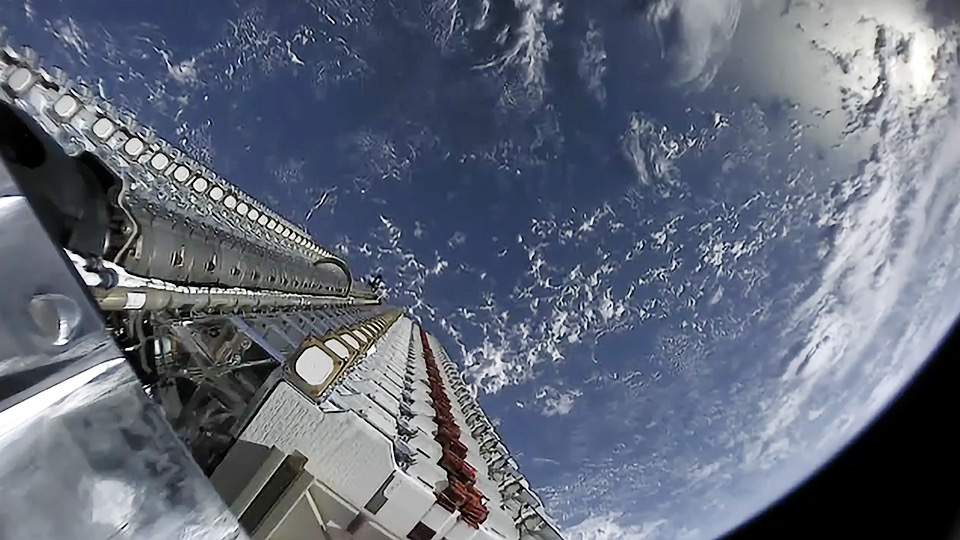
\includegraphics[width=\textwidth]{LaTeX/Figures/Starlink_cluster.jpg}
        \caption{A cluster of Starlink satellites. From~\cite{wikimedia_starlink_mission_2020}.}
        \label{fig:starlink_cluster}
    \end{subfigure}\hfill % No blank line between subfigures
    % Second subfigure (right image)
    \begin{subfigure}[b]{0.49\textwidth}
        \centering
        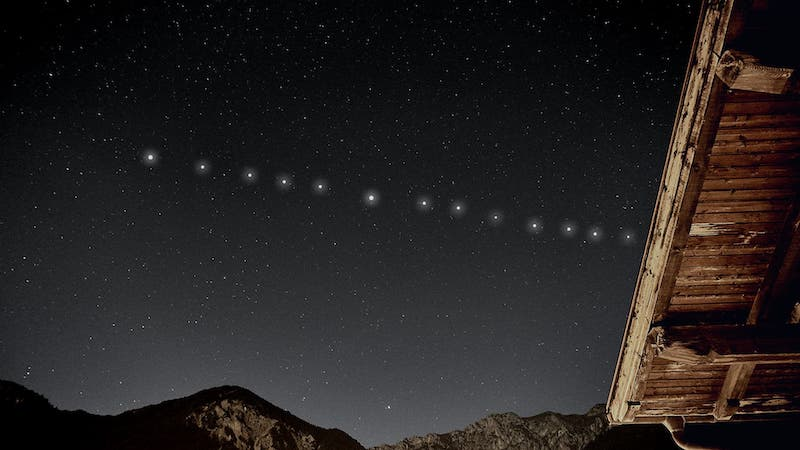
\includegraphics[width=\textwidth]{LaTeX/Figures/SPACEX-STARLINK-SATELLITES-CONSTELLATION.jpeg}
        \caption{A line of Starlink satellites. From~\cite{earthsky_starlink_2021}.}
        \label{fig:starlink_line}
    \end{subfigure}
    
\end{figure}

This project aims to investigate the orbit of an active, Earth-orbiting Starlink satellite through empirical observation and data collection. The satellite chosen is the \textit{Starlink-3988} unit, a v1.5 model as shown in Figure~\ref{fig:satellite_render}: although there aren't any attributes that distinguish it from others in the Starlink constellation, it was selected due to its favourable visibility and consistent orbital passes over Princeton, New Jersey, during the observation window (October 19–22, 2025). Furthermore, the satellite’s low-Earth orbit (LEO) characteristics, including a near-circular path, moderate inclination, and short orbital period, make it ideal for this project's requirements. A detail of the satellite's antennas is shown in Figure~\ref{fig:satellite_antennas}, and relevant attributes are reported in Table~\ref{tab:starlink3988_params}.

\begin{figure}[h!]
    \centering

    % First subfigure (left image)
    \begin{subfigure}[b]{0.49\textwidth}
        \centering
        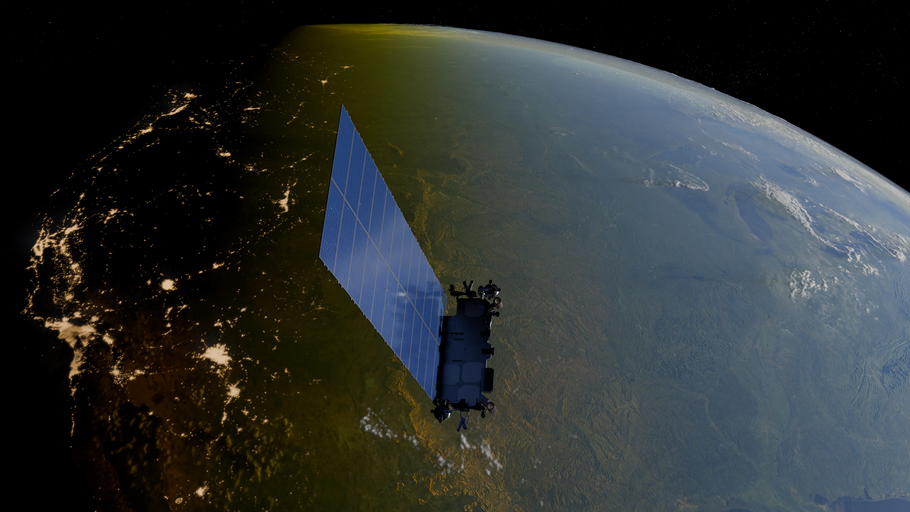
\includegraphics[width=\textwidth]{LaTeX/Figures/satellite_render.png}
        \caption{3D render of a Starlink v1.5 satellite~\cite{wikimedia_starlink_01_2025}.}
        \label{fig:satellite_render}
    \end{subfigure}\hfill % No blank line between subfigures
    % Second subfigure (right image)
    \begin{subfigure}[b]{0.49\textwidth}
        \centering
        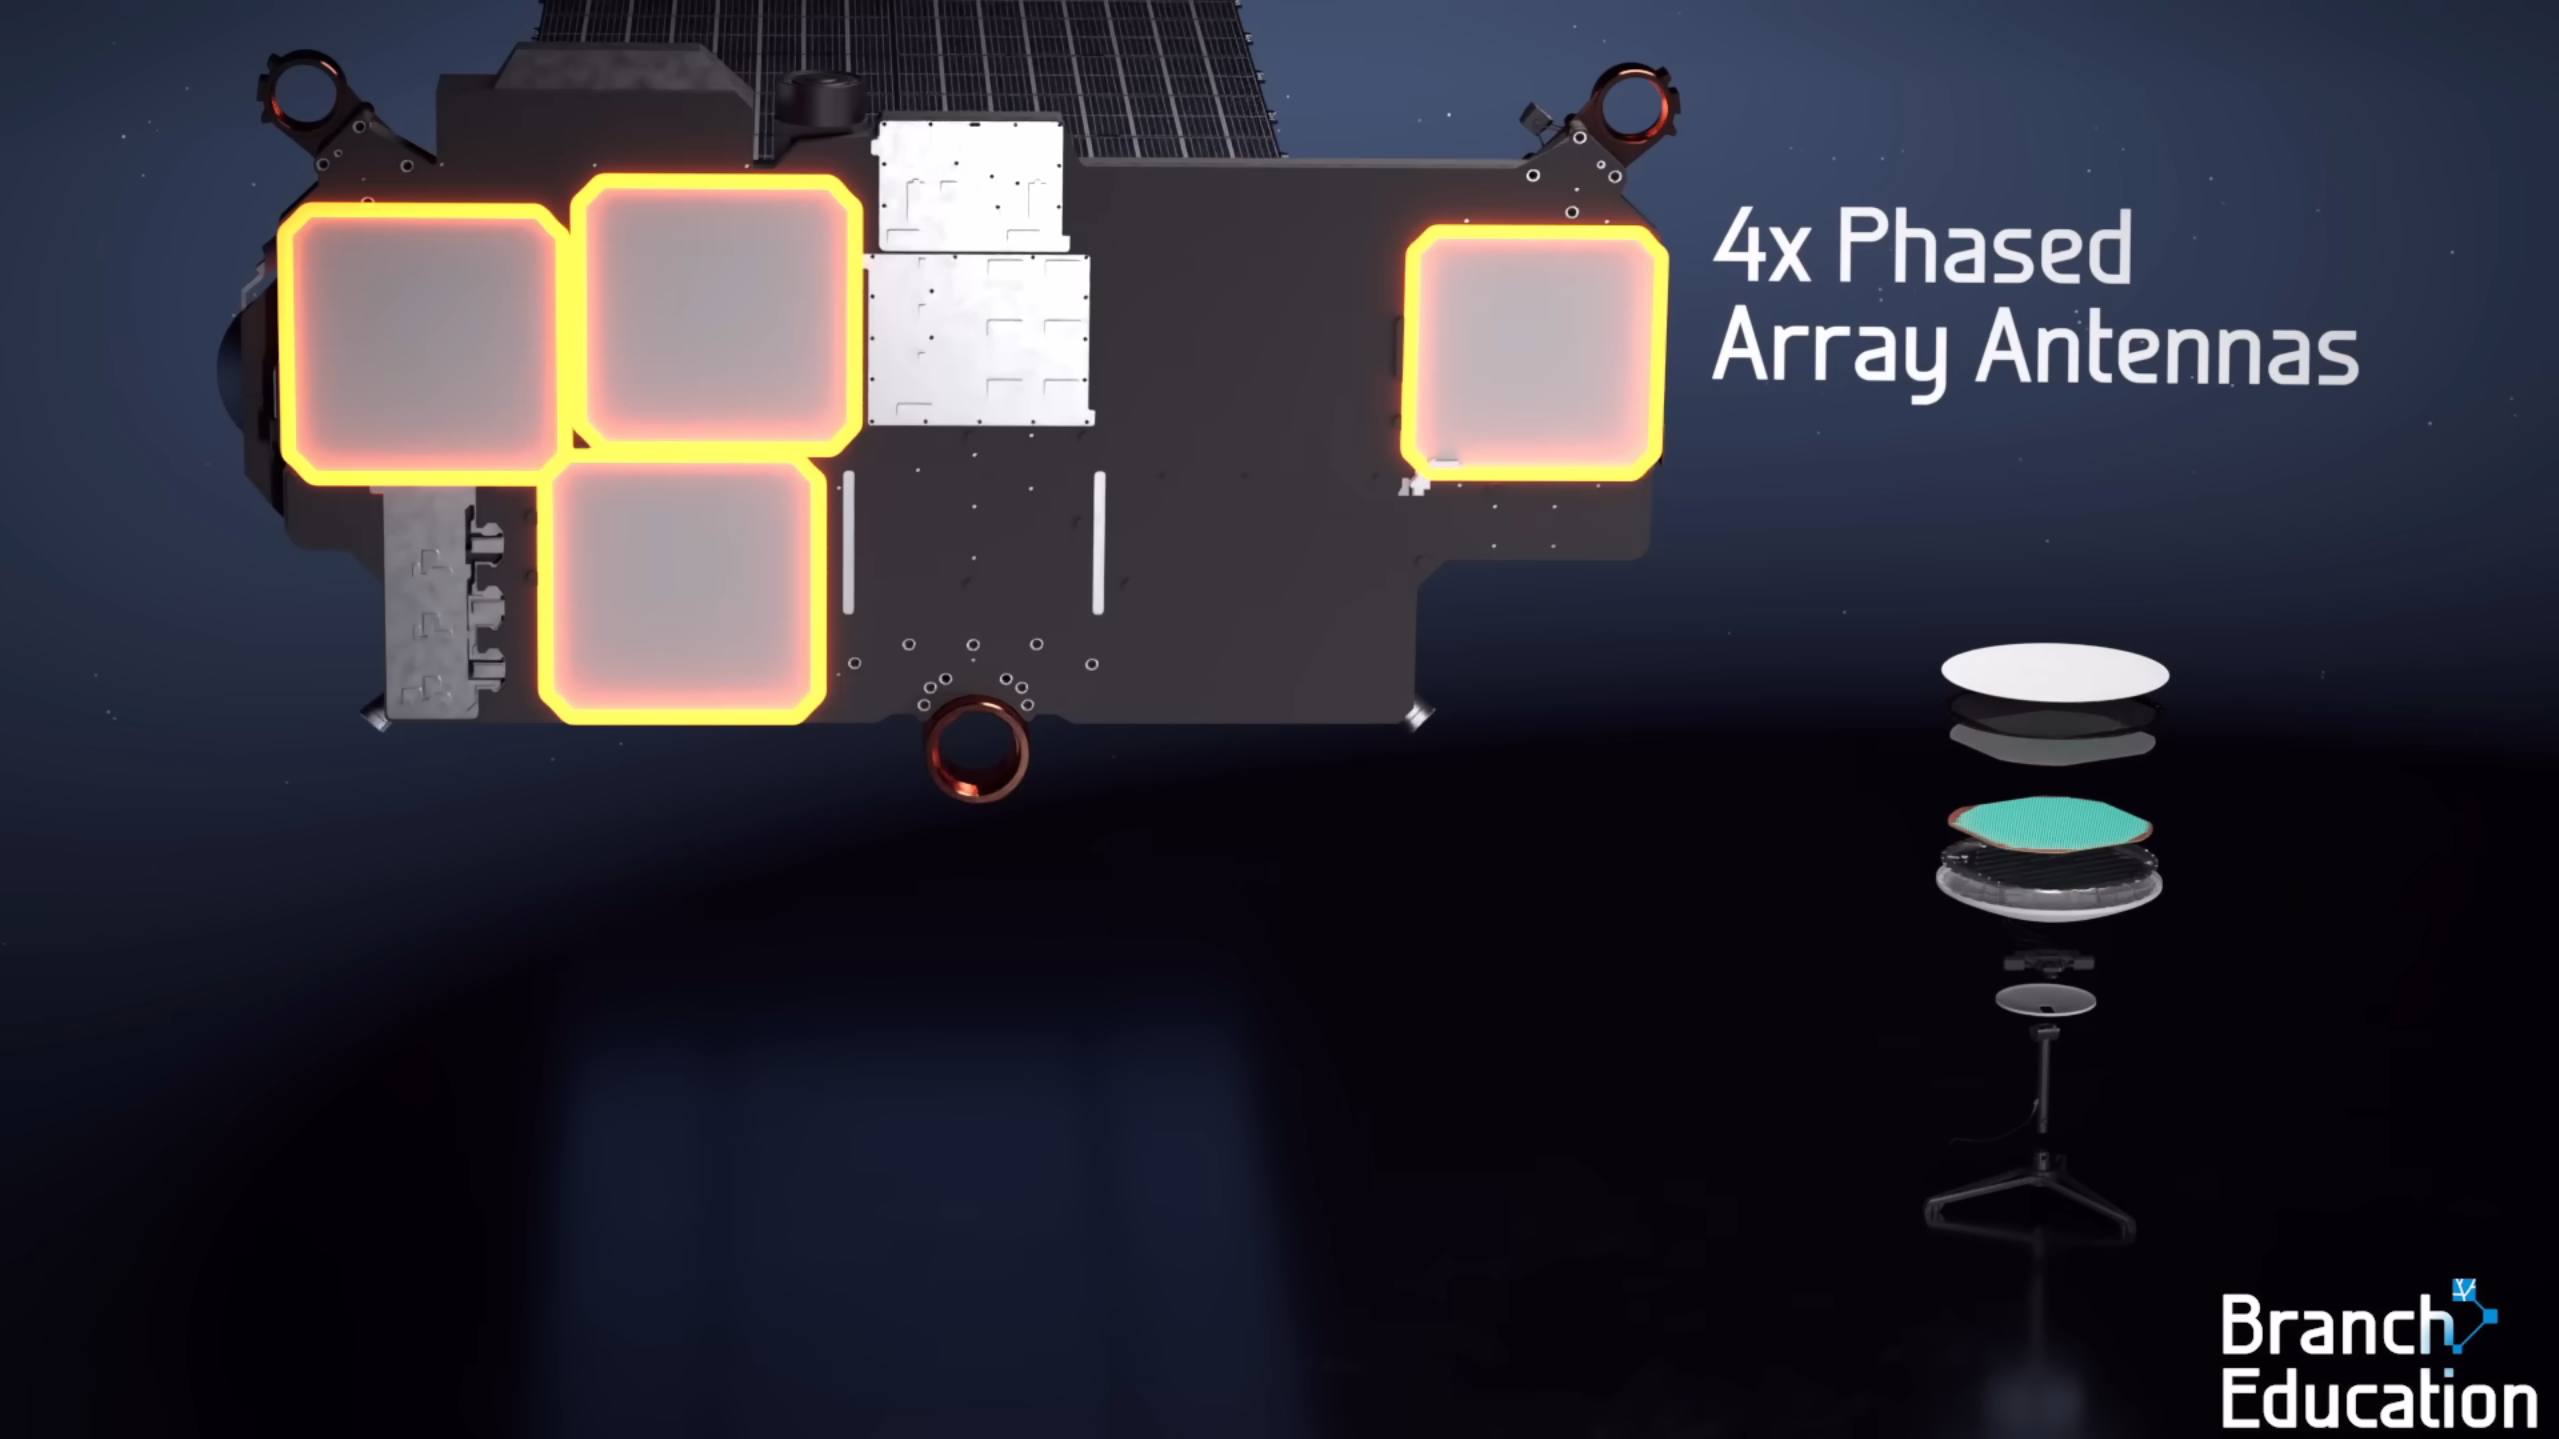
\includegraphics[width=\textwidth]{LaTeX/Figures/satellite_antennas.png}
        \caption{Satellite's antennas and dish. From~\cite{branch_education_starlink_2022}.}
        \label{fig:satellite_antennas}
    \end{subfigure}
    
\end{figure}

\begin{table}[h]
    \centering
    \caption{Key parameters for the selected satellite \textit{Starlink-3988} (NORAD ID 52625) as of October 2025. Data sourced from N2YO~\cite{n2yo_starlink3988}, In-The-Sky~\cite{inthesky_starlink3988}, StarlinkMap~\cite{starlinkmap.org}, and SpaceX public technical documentation~\cite{spacex_starlink_specs}.}
    \label{tab:starlink3988_params}
    \begin{tabular}{|l|c|c|}
        \hline
        \textbf{Parameter} & \textbf{Symbol / Unit} & \textbf{Value} \\ \hline
        NORAD Catalog Number & -- & 52625 \\ \hline
        COSPAR ID & -- & 2022-052AD \\ \hline
        Launch Date & -- & May 14, 2022 \\ \hline
        Launch Vehicle / Site & -- & Falcon 9 / Cape Canaveral (AFETR) \\ \hline
        Orbit Type & -- & Low Earth Orbit (LEO) \\ \hline
        Operational Status & -- & Active \\ \hline
        Starlink Model & -- & v1.5 (Laser Inter-satellite Links) \\ \hline
        Dimensions & -- & \SI{2.8}{\metre} $\times$ \SI{1.4}{\metre} $\times$ \SI{0.2}{\metre} (without solar array) \\ \hline
        Mass & $m$ (\si{\kilo\gram}) & 295 \\ \hline
        Inclination & $i$ (\si{\degree}) & 53.2 \\ \hline
        Semi-Major Axis & $a$ (\si{\kilo\metre}) & 6917 \\ \hline
        Perigee Altitude & $r_p$ (\si{\kilo\metre}) & 545.9 \\ \hline
        Apogee Altitude & $r_a$ (\si{\kilo\metre}) & 547.9 \\ \hline
        Mean Altitude & $h$ (\si{\kilo\metre}) & 546.9 \\ \hline
        Eccentricity & $e$ & 0.00014 \\ \hline
        Orbital Period & $T$ (\si{\minute}) & 95.4 \\ \hline
        Mean Motion & $n$ (\si{rev/day}) & 15.09 \\ \hline
    \end{tabular}
\end{table}


\newpage
\section{Data Collection}

The observations of \textit{Starlink-3988} were performed over three separate passes above Princeton, New Jersey, between 19 and 21 October 2025, using a combination of digital and visual tracking techniques. Data collection employed the \textit{Satellite Tracker} mobile application (Vito Technology) for live positioning and elevation angles, supplemented by the \textit{Heavens Above} website for verification of pass times and trajectory predictions. Each observation session consisted of recording the time, azimuth, and elevation angle at fixed reference points as the satellite traversed the sky. Screenshots of the tracking interface were captured as supporting evidence of measurement. All times were logged in Eastern Daylight Time (EDT) and later converted to UTC for consistency. Weather conditions and horizon obstructions were noted when relevant. This approach ensured sufficient temporal accuracy to support later calculations of orbital period and angular velocity, while allowing for a consistent measurement procedure across multiple sessions. Minor limitations included atmospheric haze, variable signal strength, and the finite angular precision of the mobile tracking display.

\begin{table}[H]
\centering
\caption{Raw Observational Data and Coordinate-Shifted Data}
\renewcommand{\arraystretch}{1.2}
\begin{tabular}{|c|c|c|c|c|c|}
\hline
\textbf{Date} & \textbf{Time} & \textbf{Azimuth} & \textbf{Elevation} & \textbf{Right} & \textbf{Declination} \\ 
\textbf{ } & \textbf{ } & \textbf{(°)} & \textbf{Angle (°)} & \textbf{Ascension (°)} & \textbf{(°)} \\ \hline
\multicolumn{6}{|c|}{\textbf{Observation 1 – 19 October 2025}} \\ \hline
10/19 & 19:39:15 & 321.0 & 10.0 & 189.3 & 43.8 \\ \hline
10/19 & 19:40:00 & 324.5 & 13.9 & 189.5 & 49.3 \\ \hline
10/19 & 19:41:00 & 333.4 & 21.7 & 188.3 & 60.8 \\ \hline
10/19 & 19:42:00 & 350.5 & 32.1 & 175.8 & 78.7 \\ \hline
10/19 & 19:43:00 & 024.8 & 41.0 & 029.8 & 71.3 \\ \hline
10/19 & 19:44:00 & 061.3 & 37.0 & 023.0 & 43.0 \\ \hline
10/19 & 19:45:00 & 084.6 & 26.1 & 022.3 & 20.4 \\ \hline
10/19 & 19:46:00 & 096.2 & 16.9 & 022.8 & 06.3 \\ \hline
10/19 & 19:46:29 & 102.5 & 10.2 & 023.8 & -03.7 \\ \hline
\multicolumn{6}{|c|}{\textbf{Observation 2 – 20 October 2025}} \\ \hline
 &  &  &  &  &  \\ \hline
 &  &  &  &  &  \\ \hline
 &  &  &  &  &  \\ \hline
 &  &  &  &  &  \\ \hline
\multicolumn{6}{|c|}{\textbf{Observation 3 – 21 October 2025}} \\ \hline
 &  &  &  &  &  \\ \hline
 &  &  &  &  &  \\ \hline
 &  &  &  &  &  \\ \hline
 &  &  &  &  &  \\ \hline
\end{tabular}
\end{table}

% \begin{table}[H]
% \centering
% \caption{Raw Observational Data and Coordinate-Shifted Data}
% \renewcommand{\arraystretch}{1.2}
% \begin{tabular}{|c|c|c|c|c|c|c|}
% \hline
% \textbf{Date} & \textbf{Time} & \textbf{Azimuth} & \textbf{Elevation} & \textbf{Distance} & \textbf{Right} & \textbf{Declination} \\ 
% \textbf{ } & \textbf{ } & \textbf{(°)} & \textbf{Angle (°)} & \textbf{(km)} & \textbf{Ascension (°)} & \textbf{(°)} \\ \hline
% \multicolumn{7}{|c|}{\textbf{Observation 1 – 19 October 2025}} \\ \hline
% 10/19 & 19:39:15 & 321.0 & 09.7 & 189.3 & 43.8 &  \\ \hline
% 10/19 &  &  &  &  &  &  \\ \hline
% 10/19 &  &  &  &  &  &  \\ \hline
% 10/19 &  &  &  &  &  &  \\ \hline
% \multicolumn{7}{|c|}{\textbf{Observation 2 – 20 October 2025}} \\ \hline
%  &  &  &  &  &  &  \\ \hline
%  &  &  &  &  &  &  \\ \hline
%  &  &  &  &  &  &  \\ \hline
%  &  &  &  &  &  &  \\ \hline
% \multicolumn{7}{|c|}{\textbf{Observation 3 – 21 October 2025}} \\ \hline
%  &  &  &  &  &  &  \\ \hline
%  &  &  &  &  &  &  \\ \hline
%  &  &  &  &  &  &  \\ \hline
%  &  &  &  &  &  &  \\ \hline
% \end{tabular}
% \end{table}



\section{Estimate of Period and Angular Velocity}

\section{Estimate of Semi-Major Axis and Position Prediction}

\section{Estimate of Orbital Elements}

\section{Error Analysis}

\section{Conclusion}

\section{Visualisation}

\printbibliography

\end{document}
